%   Copyright (C) 2014  School of Information Sciences, Manipal



\newcommand{\projecttitle}{Boot-Time Optimization for Android on Intel Atom Architecture}
\newcommand{\projectauthors}{\normalsize Aurabindo J}
\newcommand{\institutename}{School of Information Sciences}
\newcommand{\university}{Manipal University, Manipal}
\newcommand{\rollno}{141021001}
\documentclass{mainreport}
%\linespread{1.5}
\usepackage{hyperref}
\usepackage{makeidx}
\usepackage{multirow}
\usepackage{nomencl}
\usepackage{pdfpages}
\usepackage{subcaption}
\usepackage{tabularx}
\usepackage{listings}
\usepackage{color}
\usepackage{upquote}
\usepackage{relsize}
\usepackage{fancyvrb}
%\usepackage{biblatex}

\definecolor{dkgreen}{rgb}{0,0.6,0}
\definecolor{gray}{rgb}{0.5,0.5,0.5}
\definecolor{mauve}{rgb}{0.58,0,0.82}


\lstset{frame=tb,
  aboveskip=3mm,
  belowskip=3mm,
  showstringspaces=false,
  columns=flexible,
  basicstyle={\small\ttfamily},
  numbers=none,
  numberstyle=\tiny\color{gray},
  keywordstyle=\color{blue},
  commentstyle=\color{dkgreen},
  stringstyle=\color{mauve},
  breaklines=true,
  breakatwhitespace=true
  tabsize=3
}

%\usepackage{tocloft}


\newcommand{\tab}{\hspace*{2em}}
% for removing dots

\makeatletter
\renewcommand{\@dotsep}{10000} 
\makeatother

\renewcommand{\figurename}{Fig.}


\begin{document}

\maketitle
%\makecertificate

\parindent 10mm
%\newgeometry{bottom=2.5cm,top=2.5cm}
\chapter*{Acknowledgment}\label{ack}\addcontentsline{toc}{chapter}{Acknowledgment}
{\label{ack} 

%\paragraph*{•}
\hspace{6mm} This project itself is an acknowledgment to the inspiration, drive and technical
assistance contributed by many individuals. I would like to express my heartfelt thanks to my project guides 
{\bf Dr. Harishchandra Hebbar} and {\bf Dr. Nandish Rao}
%\paragraph*{•}
I would like to thank all the teaching and non teaching faculties of {\bf School of Information Sciences}, 
in particular, for providing us with an ample environment and
infrastructure required to carry out this project. 

This project would not be possible without the support from {\bf Intel India}. I thank \
{\bf Mr. Satish A Hipparagi}, and {\bf Mr. Abhilash K.V.}, engineers at Intel,
for the inspiration and support rendered.

%\paragraph*{•}
I extend my heartfelt thanks to my parents, friends and well wishers for their 
support and timely help. Above all I thank the Almighty for His blessing and 
providing mercies at all stages of my work. \\[2cm]




\noindent Manipal \hfill Project Members

\noindent \today \hfill \institutename

 \hfill Manipal





}

\chapter*{Abstract}\label{Abstract}\addcontentsline{toc}{chapter}{Abstract}

{
\label{Abstract}



%\paragraph*{•}
\hspace{6mm} When Android framework was getting developed, systems using ARM core and
corresponding sub system architecture were widely used. As the ARM ecosystem evolved,
it established itself as one of the leading vehicle for Android platform. Consequently,
Android ecosystem also developed around ARM architecture including application
development, services and even system level optimization. When x86 core also entered
this Android ecosystem, effort was put in to make system level optimization for
Android products based on x86 Architecture.

This thesis aims at evaluating various known methods as well as finding new areas
for optimization. Optimization effort will be targeting at reducing the boot time of
the the system by evaluating various components which includes BIOS firmware,
Bootloader, Linux Kernel and other AOSP components.
%\end{center}
}

%generate table of contents
\tableofcontents

%\chapter*{List of Symbols}\label{symbol}\addcontentsline{toc}{chapter}{List of Symbols}
%\listofsymbols

%\input{symbol}

%\input{fig}

\listoffigures
\addcontentsline{toc}{chapter}{List of Figures}
%\listoftables
\addtocontents{lof}{\textbf{No.}\hspace{8 mm}\textbf{Figure}~\hfill\textbf{Page}\par}
%\newpage


\chapter*{List of Abbreviations}\label{abbrv}\addcontentsline{toc}{chapter}{List of Abbreviations}




%Add your abbreviations here as follows
%\nomenclatue{Abbr}{Abbreviation}
%Example:
%\makenomenclature
\begin{center}
\label{abbrv}
\begin{tabular}{r l}
	TTYL & Talk To You Later \\
	AFAIK & As Far As I Know \\
	IMHO & In My Humble Opinion \\
	IMO & In My Opinion (not so humble)\\
	ROFL & Rolling On The Floor and Laughing
\end{tabular}
\end{center}


\newpage



%\chapter*{Report}\label{report}\addcontentsline{toc}{chapter}{Report}

\pagenumbering{arabic}



\section{Introduction}
\label{report}


\hspace{8mm} 

\noindent Mobile devices are the one of the most competitive consumer technology equipment market.
Manufacturers come up with improved or advanced versions of their product quite sooner that
people expect. With the demand from the market for more of performance, features, battery
life, etc the need to optimizing existing products also arise. Hence optimization of boot time
for Android devices are quite relevant.

We will look into the overview of Android booting sequence from all levels. Then we will look
deeply into available tools to evaluate the boot time. Various profiling tools which help understand
the booting process in detail will also be covered in detail. Finally we will look at the techniques
and procedures which will help in reducing the boot time. The optimizing effort will be focused on the
linux kernel and bootloader.

\subsection{About Android}

Android is an open source mobile OS currently developed by Google, based on the Linux kernel and designed
primarily for touchscreen mobile devices such as smartphones and tablets. Initially developed
by Android, Inc., which Google bought in 2005. Android was unveiled in 2007, along with the
founding of the Open Handset Alliance – a consortium of hardware, software, and telecommunication
companies devoted to advancing open standards for mobile devices. However, most Android devices
ultimately ship with a combination of open source and proprietary software, including proprietary
software required for accessing Google services.


Linux kernel is the core part of the Android OS. The version of the linux kernel used in Android is
based on one of the Linux kernel's LTS branches. Android's variant of the Linux kernel has further
architectural changes that are implemented by Google outside the typical Linux kernel development
cycle, such as the inclusion of components like Binder, ashmem, pmem, logger, wakelocks,
and different out-of-memory (OOM) handling.

\subsubsection {Hardware}

The main hardware platform for Android is the ARM architecture (ARMv7 and ARMv8-A architectures),
with x86 and MIPS architectures also officially supported in later versions of Android.
Since Android 5.0 "Lollipop", 64-bit variants of all platforms are supported in
addition to the 32-bit variants.

Intel has its processors specifically made for low power devices, which run Android.
This architecture is known as Intel Atom. It is a SoC which offers good performance with
reduced power consumption compared to a full fledged desktop processors known under
the series Intel Core.

\subsubsection{Software Stack}

On top of the Linux kernel, there are the middleware, libraries and APIs written in C,
and application software running on an application framework which includes
Java-compatible libraries based on Apache Harmony. Development of the Linux kernel
continues independently of other Android's source code bases.

\begin{figure}[h]
  \centering
    \centering
    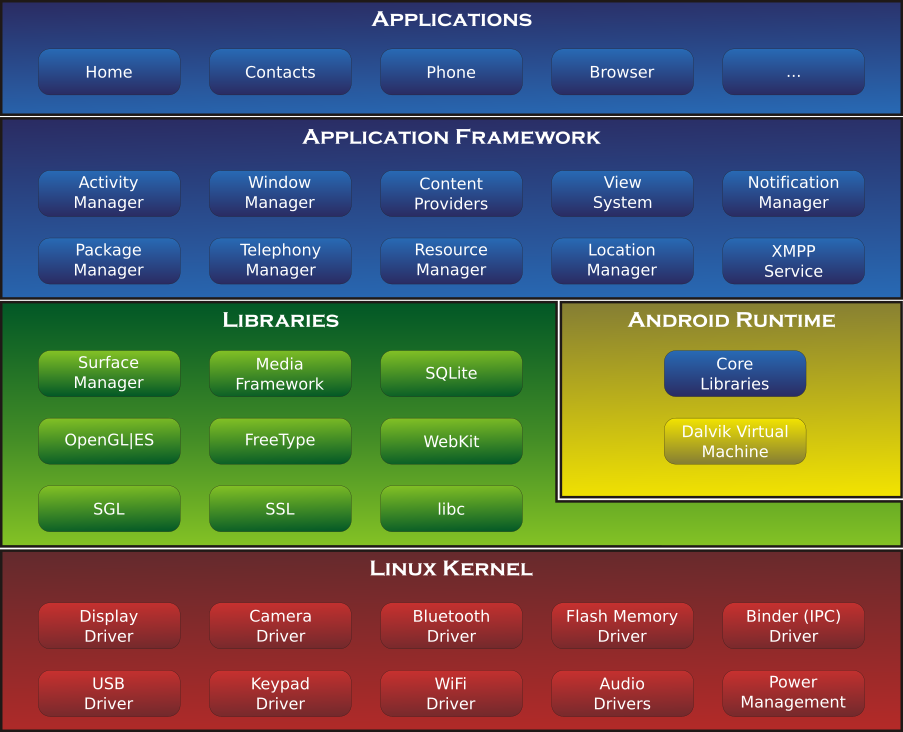
\includegraphics[scale=0.6]{android_arch.png}
    \caption{Android Software Architecture}
    \label{fig:android_arch}
\end{figure}

%\begin{figure}[h!]
%  \centering
%    	\includegraphics[scale=0.5]{scada_architecture.png}
%	\caption{Architecure of a typical power SCADA system}
%	\label{scada_arch} %the label was cycle here



%\begin{figure}[h]
%  \centering
%  \begin{subfigure}[b]{1\textwidth}
%    \centering
%    \includegraphics[scale=0.4]{digraph_simple.png}
%    \caption{relation digraph of the simplified system}
%    \label{fig:digraph_simple}
%  \end{subfigure}
  
%  \begin{subfigure}[b]{1\textwidth}
%    \centering
%    \includegraphics[scale=0.4]{digraph_virtual.png}
%    \caption{Representation of the digraph with virtual nodes}
%    \label{fig:digraph_virtual}
%  \end{subfigure}
  
%\end{figure}




\section{Android Boot Sequence}
\label{android_boot}


\hspace{8mm} 

\noindent At the core of Android is the Linux Kernel managing all the underlying hardware. Hence boot process is
similar to what we find in a Linux machine. However, the devices which run Android are highly
integrated devices, called SoCs, which have a wide range of devices which we dont find in
a normal linux desktop system or a laptop. Much of these devices come with proprietary drivers.
The bootloader usually used for ARM based SoCs, is called Uboot. However, for Intel Atom SoC
based on the Cherrytrail family uses a proprietary bootloader, called Kernelflinger.

Once Kernel is started, it does the driver initialization and call the first userspace program,
called init. From here, what init loads is making the difference as what we see Android as it is.

The diagram below shows the boot flow in Android:


\begin{figure}[h]
  \centering
    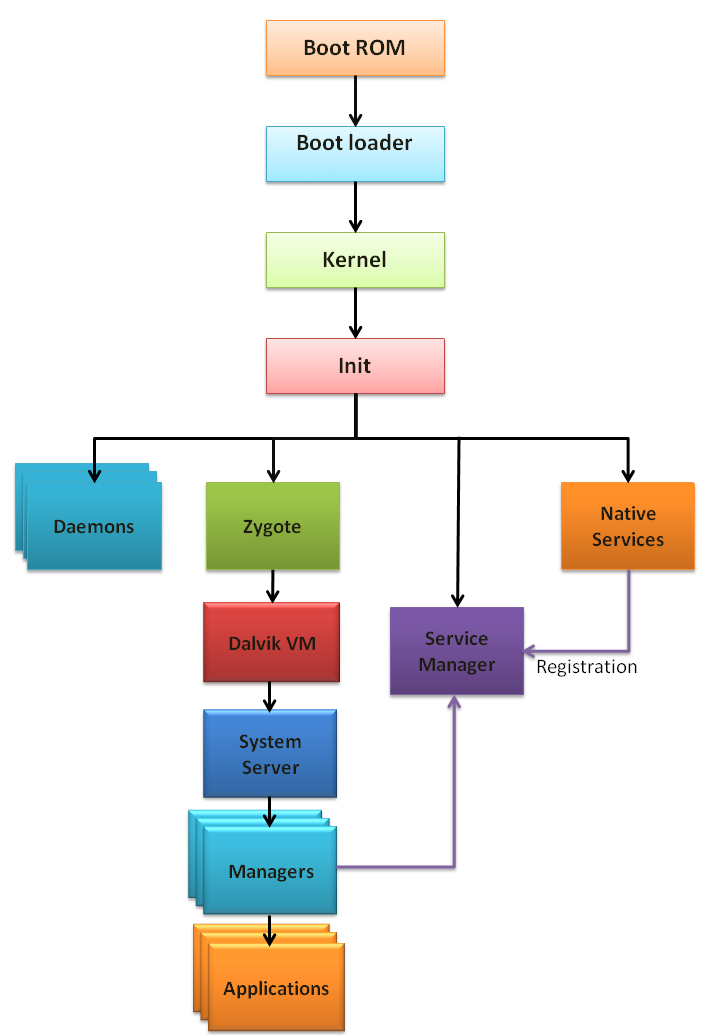
\includegraphics[scale=0.7]{android_boot.png}
    \caption{Android Boot Process}
    \label{fig:android_boot}
\end{figure}

\clearpage
\subsection{Bootloader}

Up on power up, the SoC firmware boots from a ROM area typically located internally,
different from the system's eMMC card. This is what we loosely call BIOS, for legacy
reasons. This code determines the boot media and loads the boot loader from the media.
The boot loader can be used to initialize the DRAM and load another level of loader
or directly the Linux kernel. On Cherrytrail Platform, the bootloader is called Kernelflinger.
It then loads the Linux Kernel with the required parameters hardcoded in the boot image.

\subsection{Kernel}

Linux kernel is the heart of the Android responsible for the process creation, inter process communication, device drivers, file system management etc. Android applies a custom patch on the main stream kernel to support certain features like Wake locks etc needed for operation of the Android.

The kernel is loaded as a compressed imaege. Up on loading, it decompresses itself,
does the driver initializations, mounts the root file system (typically passed 
as kernel command line arguments) and starts the first application in user space.


\subsection{Android}

Android typically operates wholly on the user space. The android applications are executed over a Virtual Machine called the Dalvik. The following section explains the internals in detail.

\subsubsection{init and init.rc}

The first user space application executed on booting the kernel is the init
executable located in the root folder. The process parses a start up script
called the \textit{init.rc} script. This is written in a language designed
for android used to start all the necessary processes, daemons and services
for a proper operation of android. It offers various types of execution timings
such as early-init, on-boot, on-post-fs etc. A detailed explanation of the
scripting model is available on Android documentation site.

\subsubsection{Demons and Services}

The init process creates various daemons and processes like rild, vold,
mediaserver, adb, etc each responsible for its own functionality.
Descriptions of these processes are not in the scope of this post.
Rather we will discuss more about \textit{Zygote} process.

\subsubsection{Service Manager}

The service manager process manages all the services running in the system.
Every service created registers itself with this process and this information
is used for future references by other processes/applications.

\subsubsection{Zygote}

Zygote is one of the first init process created on boot. The term ``zygote`` is based the biological ''initial cell formed
that divides to produce offsprings``. Similarly zygote in android initializes the Dalivik VM and
forks to create multiple instances to support each android process. It facilitates using a shared code
across the VM instances resulting in a low memory foot print and short load time, ideal for an embedded system.

Zygote apart from installing a listener on the server socket, also preloads classes and
resources to be used later in the Android applications. Once done, the system server is started.

%nbegin{figure}[h]
%  \centering
%  \begin{subfigure}[b]{1\textwidth}
%    \centering
%    \includegraphics[scale=0.4]{digraph_simple.png}
%    \caption{Relation digraph of the simplified system}
%    \label{fig:digraph_simple}
%  \end{subfigure}
  
%  \begin{subfigure}[b]{1\textwidth}
%    \centering
%    \includegraphics[scale=0.4]{digraph_virtual.png}
%    \caption{Representation of the digraph with virtual nodes}
%    \label{fig:digraph_virtual}
%  \end{subfigure}
  
%\end{figure}




\section{Profiling Tools and Techniques}
\label{prof_tools_techniques}


\begin{frame}
	\frametitle{Profiling Tools and Techniques}
	\begin{itemize}
		\item Bootchart \pause
		\item Bootloader Timestamp \pause
		\item Initcall Debug \pause
	\end{itemize}
\end{frame}

\subsection{Bootchart}

\begin{frame}
\begin{figure}[h]
  \centering
    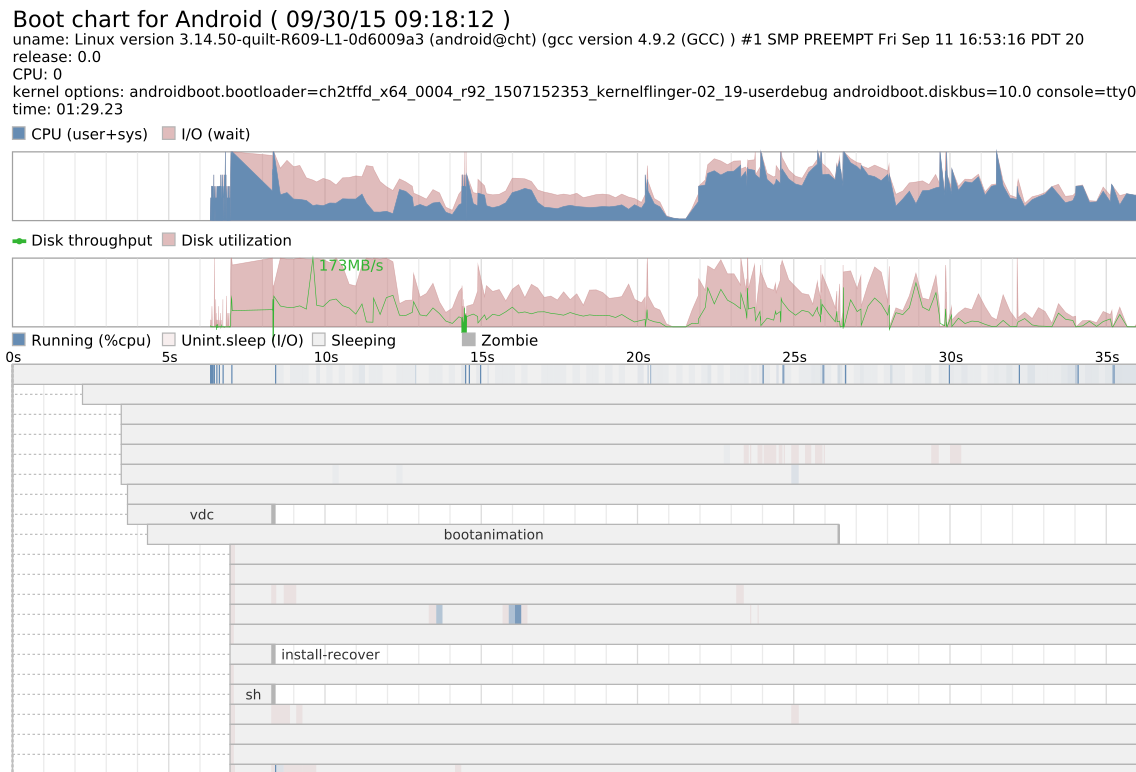
\includegraphics[scale=0.3]{bootchart.png}
    \caption{Bootchart output from Android}
    \label{fig:android_boot}
\end{figure}
\end{frame}

\subsection{Bootloader Timestamps}

\begin{frame}
	\frametitle{Profiling Tools and Techniques}
\begin{enumerate}
	\item Using UEFI {\bf GetTime()} function \pause
	\item Using Host-side serial timestamp \pause
	\item Using {\bf RDTSC} instruction \pause
\end{enumerate}
\end{frame}


\subsection {Initcall Debug}

\begin{frame}[fragile]
	\frametitle{Initcall Debug}
	\begin{itemize}
		\item Kernel command line argument \pause
		\item Trace Driver Initilization function \pause
		\item Measure Time for completion \pause
	\end{itemize}
	\begin{Verbatim}[fontsize=\small]
	dmesg -s 128000 | grep ``initcall`` | \ 
	sed ''s/\(.\)after\(.\)/\2 \1/g'' | sort -n -r
	\end{Verbatim}
\end{frame}


\begin{frame}[fragile]
	\frametitle{Sample output}
	\begin{adjustwidth}{-2em}{-2em}
\begin{Verbatim}[fontsize=\footnotesize]
322342 usecs <7>[ 1.230001] initcall i915_init+0x0/0x74 returned 0
254394 usecs <7>[ 4.872194] initcall ov8858_init_mod+0x0/0x1000 returned 0
220703 usecs <7>[ 0.455998] initcall acpi_init+0x0/0x25e returned 0
214826 usecs <7>[ 1.488846] initcall dwc3_pci_driver_init+0x0/0x1b returned 0
209263 usecs <7>[ 5.364468] initcall atomisp_init+0x0/0xd51 returned 0
199893 usecs <7>[ 0.781643] initcall populate_rootfs+0x0/0xd8 returned 0
133947 usecs <7>[ 2.253326] initcall pmic_ccsm_init+0x0/0x14 returned 0
133379 usecs <7>[ 5.121348] initcall init_lm3554+0x0/0x1000 returned 0
113899 usecs <7>[ 1.890387] initcall intel_pram_init+0x0/0x1d3 returned 0
92015 usecs <7>[  4.975765] initcall init_ov2722+0x0/0x20 returned 0
\end{Verbatim}
	\end{adjustwidth}

\end{frame}




\section{Future Work}
\label{fut_work}


\hspace{8mm} 

\noindent There are advanced tools to profile kernel drivers so as to know
where most of the time is being spent by the drivers. There are other numerous
optimizations possible in the kernel space as well as userspace.
All such discreete measurements are to be conducted.

Unfortunately it is not very straightforward to profile device drivers that are built into the kernel,
since their initialization takes place when there is no userspace ready. Hence we cannot use the normal
tools to trigger profiling. However, the system can be configured to starting tracing at the boot itself.

\subsection{Discrete Optimizations}

Some other optimization strategies that could be done are summarized below:

\subsubsection{Right CPU Frequency}

In some systems, the power consumed by the display is very high compared to
the rest of the system. Depending on the BOM, the hardware limitation in peak
current can vary. During boot time, inorded to reduce power consumption,
the CPU governor, the component which controls the frequency of the CPU
cores are sometimes not running at their full speed. This certainly helps
reduce power consumption. However, not all platforms might need such a capping.

Increasing the CPU clock frequency to a high value during early boot is a sane
way to improve the boot times. This can be achieved by using a simple
init.rc script:
\begin{verbatim}
on early-init
write /sys/devices/system/cpu/cpu0/cpufreq/scaling_max_freq 1050000
write /sys/devices/system/cpu/cpu1/cpufreq/scaling_max_freq 1050000
write /sys/devices/system/cpu/cpu2/cpufreq/scaling_max_freq 1050000
write /sys/devices/system/cpu/cpu3/cpufreq/scaling_max_freq 1050000
\end{verbatim}

\subsubsection{Enabling DMA}

Direct Memory Access is a technique to increase the data
transfer throughput such that CPU doest not interfere in the process
When we are using an application on top a kernel, copy or move operations
shall be backed by DMA and this is controlled by the kernel. 
However, when using low level code, like say, bootloader, the copy function
may not necessarily be optimized to use DMA for various data transfer
operations. This is significantly improve boot time when the system
is copying the vital components like kernel itself, since in most
cases, every other jobs will be blocked or dependent on the kernel
itslef.

\subsubsection{Read Ahead}

It is observed that a lot of time is spent waiting for I/O
when the system is booting. Read Ahead addresses this issue.
Read ahead is a technique in which commonly used files are
fetched early when the processor is busy doing computational job
which does not require the bus access. Hence the idle bus is
exploited. In an ideal read ahead implementation, a daemon should
run during every boot and check what files init is trying to access.
The daemon should adapt its fetching process to reflect the
system requirements.

\subsubsection{Group Writes}

Writes take longer than to read. This technique involves
grouping random writes. When a write operation is encountered,
it is not immediately executed. The system will wait for few more
writes until a threshold is exceeded. This threshold could either
be time based or size based. For example, all the writes for 100 ms
will be aggregated and written. That way writes happen every 100 ms
to the actual disk. For size based threshold, 10 random writes of 1 kB
might fill the threshold of 10 kB required to trigger an actual write
operation. This feature is also provided by files systems. However,
drivers also provide such a feature known as ``packed commands''

\subsubsection{File System}

Various software level optimizations can be done to make I/O
faster, which will inturn make the booting operation faster.
These include filesystem level options that can be changed.

Android uses ext4 file system. It offers lot of options to improve
the speed of I/O operations at the cost of reduced reliability.
For example, there are some of the options provided by EXT4:
\begin{itemize}
	\item \textbf{commit}: ext4 can be told to sync all its data and metadata
			every 'nrsec' seconds. The default value is 5 seconds.
			This means that if you lose your power, you will lose
			as much as the latest 5 seconds of work (your
			filesystem will not be damaged though, thanks to the
			journaling).  This default value (or any low value)
			will hurt performance, but it's good for data-safety.
			Setting it to 0 will have the same effect as leaving
			it at the default (5 seconds).
			Setting it to very large values will improve
			performance.

	\item \textbf{noatime,nodiratime}: Whenever a file is accessed (read), a
			timestamp information is also written by default. This can
			be avoided with these options. nodiratime is the similar option
			but applies to directories rather than files. With these options
			enabled, only a write operation will cause the change of timestamp
			information.
	\item \textbf{data=writeback}: EXT4 is journalling file system. \textit{data=writeback}
			disables this feature so that write performance is increased. However,
			this reduced the reliability and the data will more prone to irrecoverable
			corruption.
	\item \textbf{dioread\_nolock}: If the dioread\_nolock option is specified
			ext4 will allocate uninitialized extent before buffer
			write and convert the extent to initialized after IO
			completes. This approach allows ext4 code to avoid
			using inode mutex, which improves scalability on high
			speed storages.	
\end{itemize}




\section{Conclusion}
\label{conclusion}


\hspace{8mm} 

\noindent Many of the techniques for boot time profiling have been evaluated and with the
help of it, an overall idea of the Linux Kernel / Android boot proccess has been understood.



%\chapter*{Datasheets}\label{datasheet}\addcontentsline{toc}{chapter}{Datasheets}

%{\label{nexys3}\includepdf[pages={-}]{Nexys3_rm.pdf} 
%{\label{nexys3}\includepdf[pages={1-1,8-10,11-14,18-20}]{Nexys3_rm.pdf} 
%{\label{nexys3}\includepdf[pages={1-1}]{spartan6.pdf} 

\nocite{*}
\bibliographystyle{plain}
\bibliography{master}

\end{document}
